\section{Results}
In table \ref{tab:mse} the mean squared error (MSE) of all trained models is shown. Clearly these errors are quite low, but in the context of our regression model the error is naturally quite low, because the mean squared error is not a relative value but an absolute value and depends on the value range which, in our case, is small. 

\begin{table}[h]
	\resizebox{.65\columnwidth}{!}{%
		\centering
		\begin{tabular}{|l|c|}
			\hline
			Model & MSE \\
			\hline
			ETS & 0.005806121997238007 \\
			HGB & 0.006537057262386852 \\
			LGB & 0.006659725937704261 \\
			XGB & 0.009520274940766137 \\
			\hline
		\end{tabular}
	}
	\caption{Mean squared error of trained models}
	\label{tab:mse}
\end{table}

In the figure \ref{fig:predictions} the orange lines represent our prediction and the blue lines represent the ground truth. With these figures it is quite clear why the mean squared error value needs to be even lower.

\begin{figure*}[bt]
	\begin{subfigure}{.24\textwidth}
		\centering
		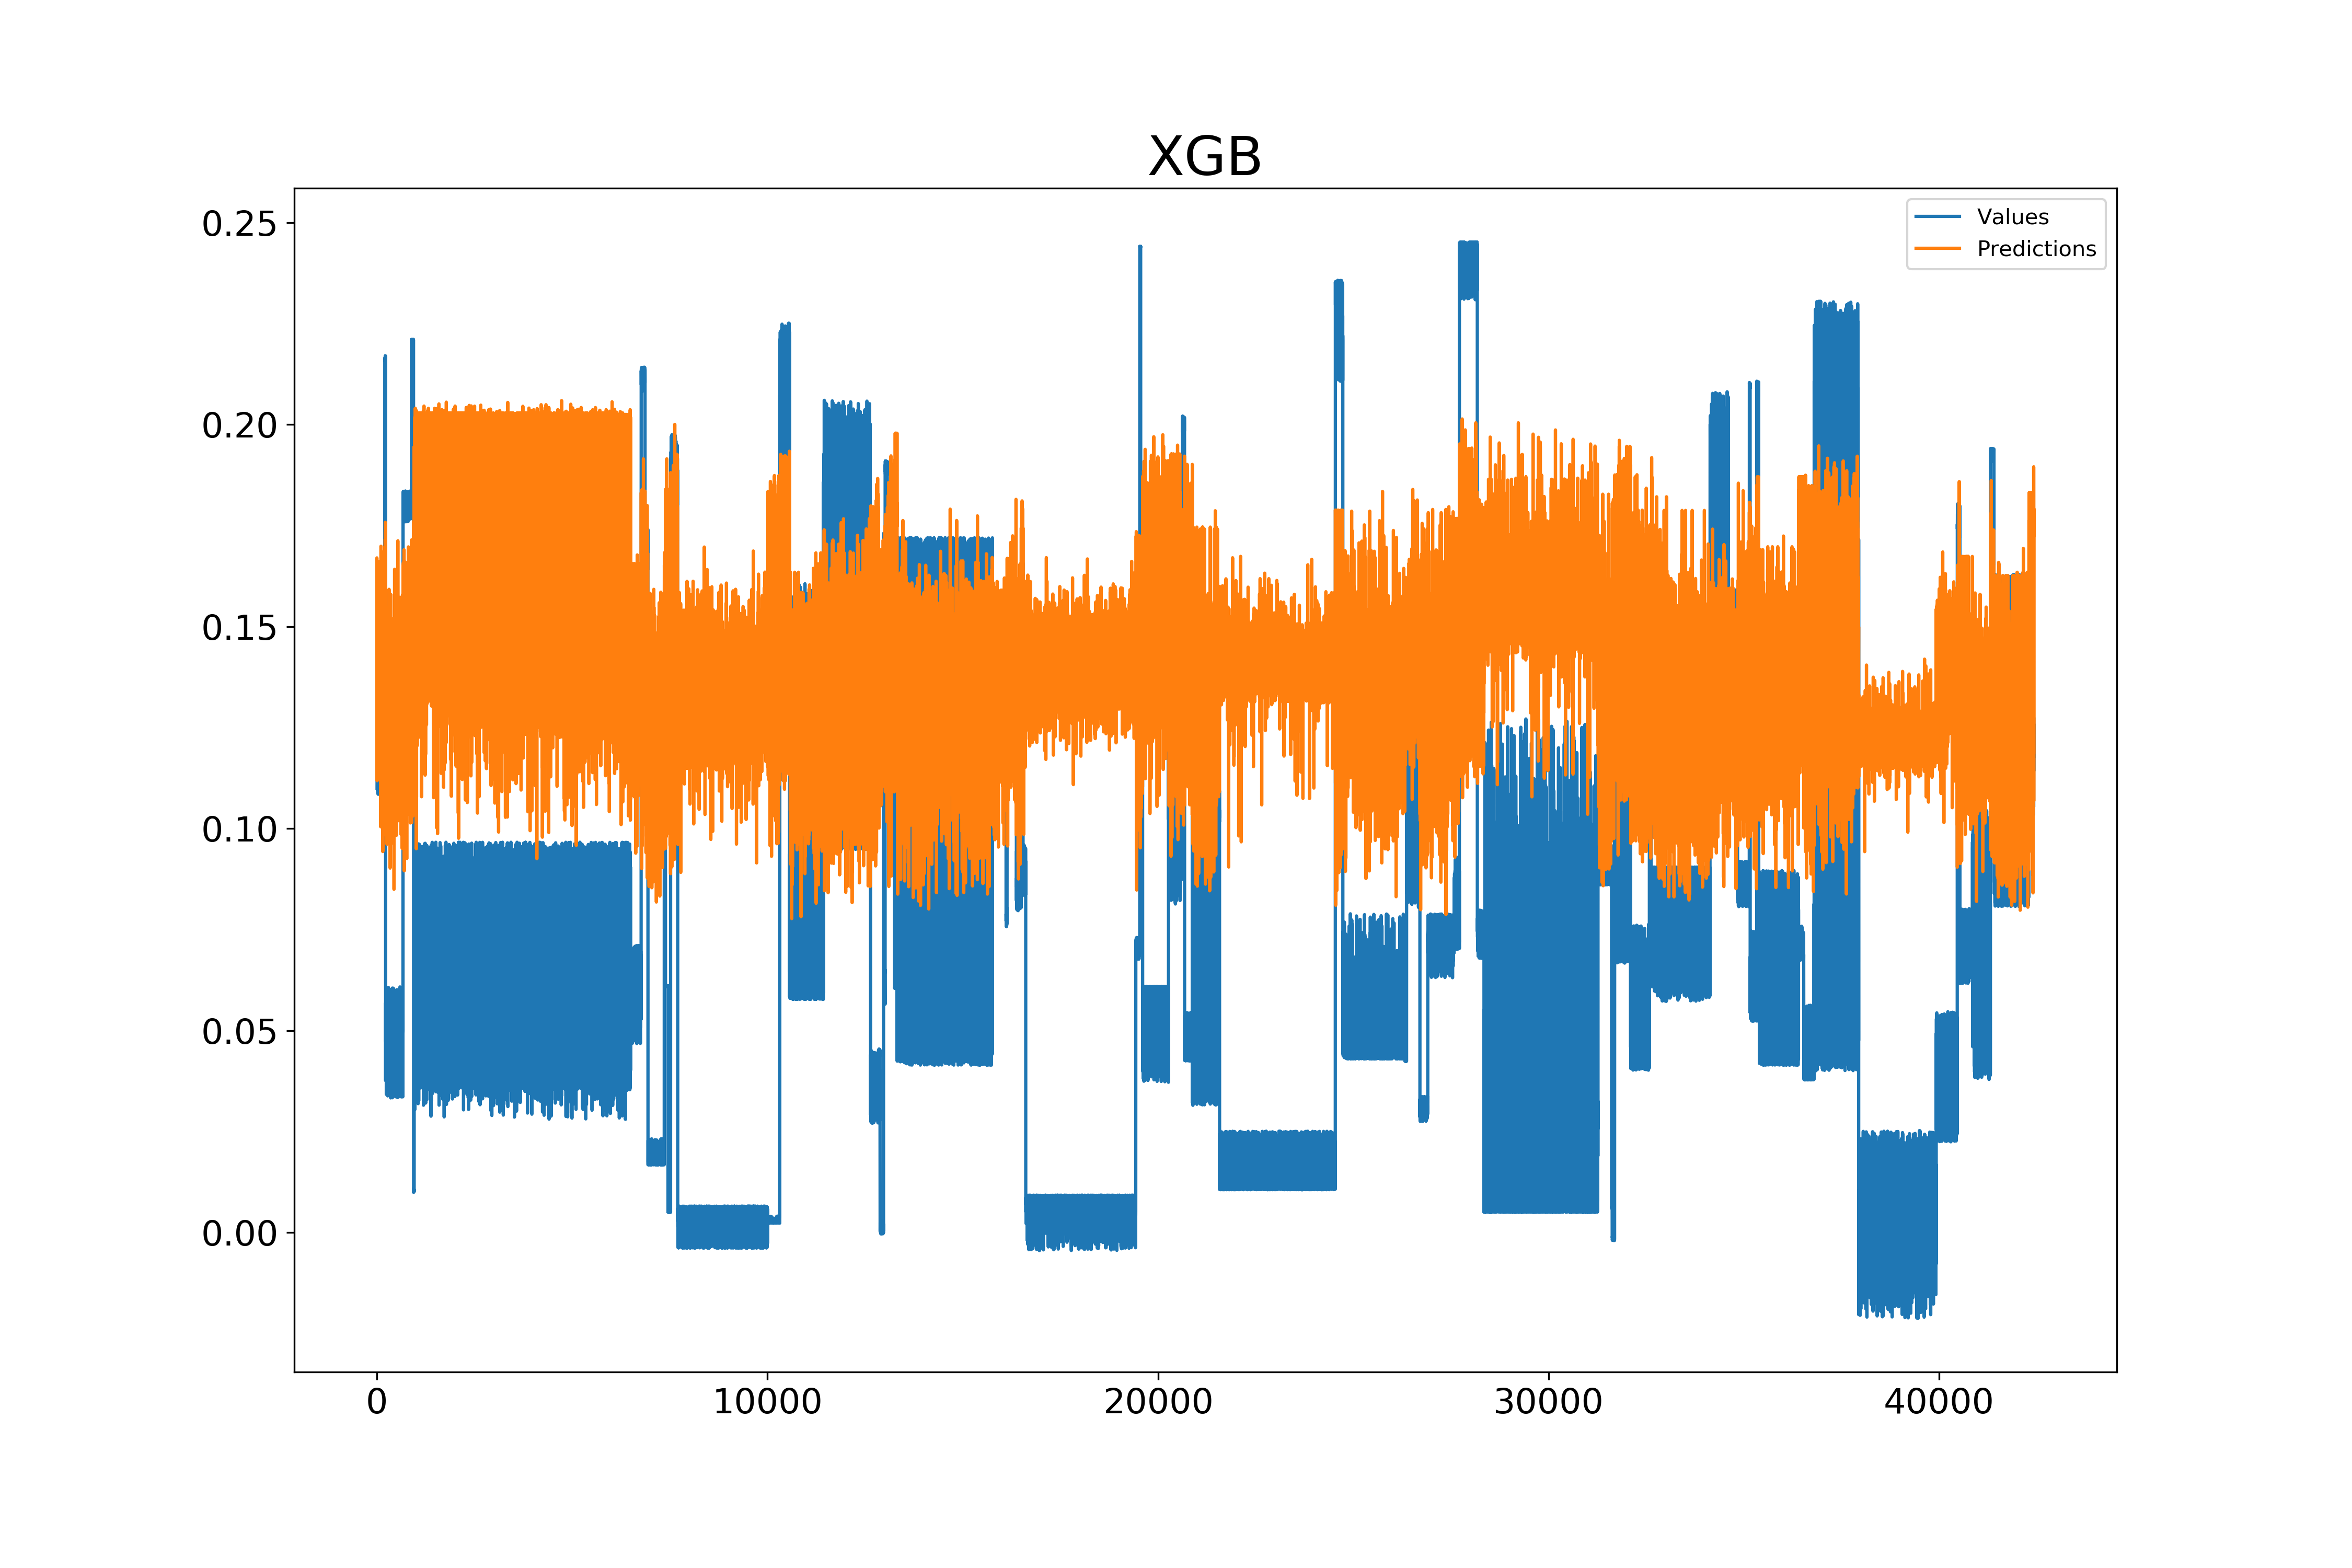
\includegraphics[width=\textwidth]{XGB_results}
		\caption{XGBoost}
	\end{subfigure}
	\begin{subfigure}{.24\textwidth}
		\centering
		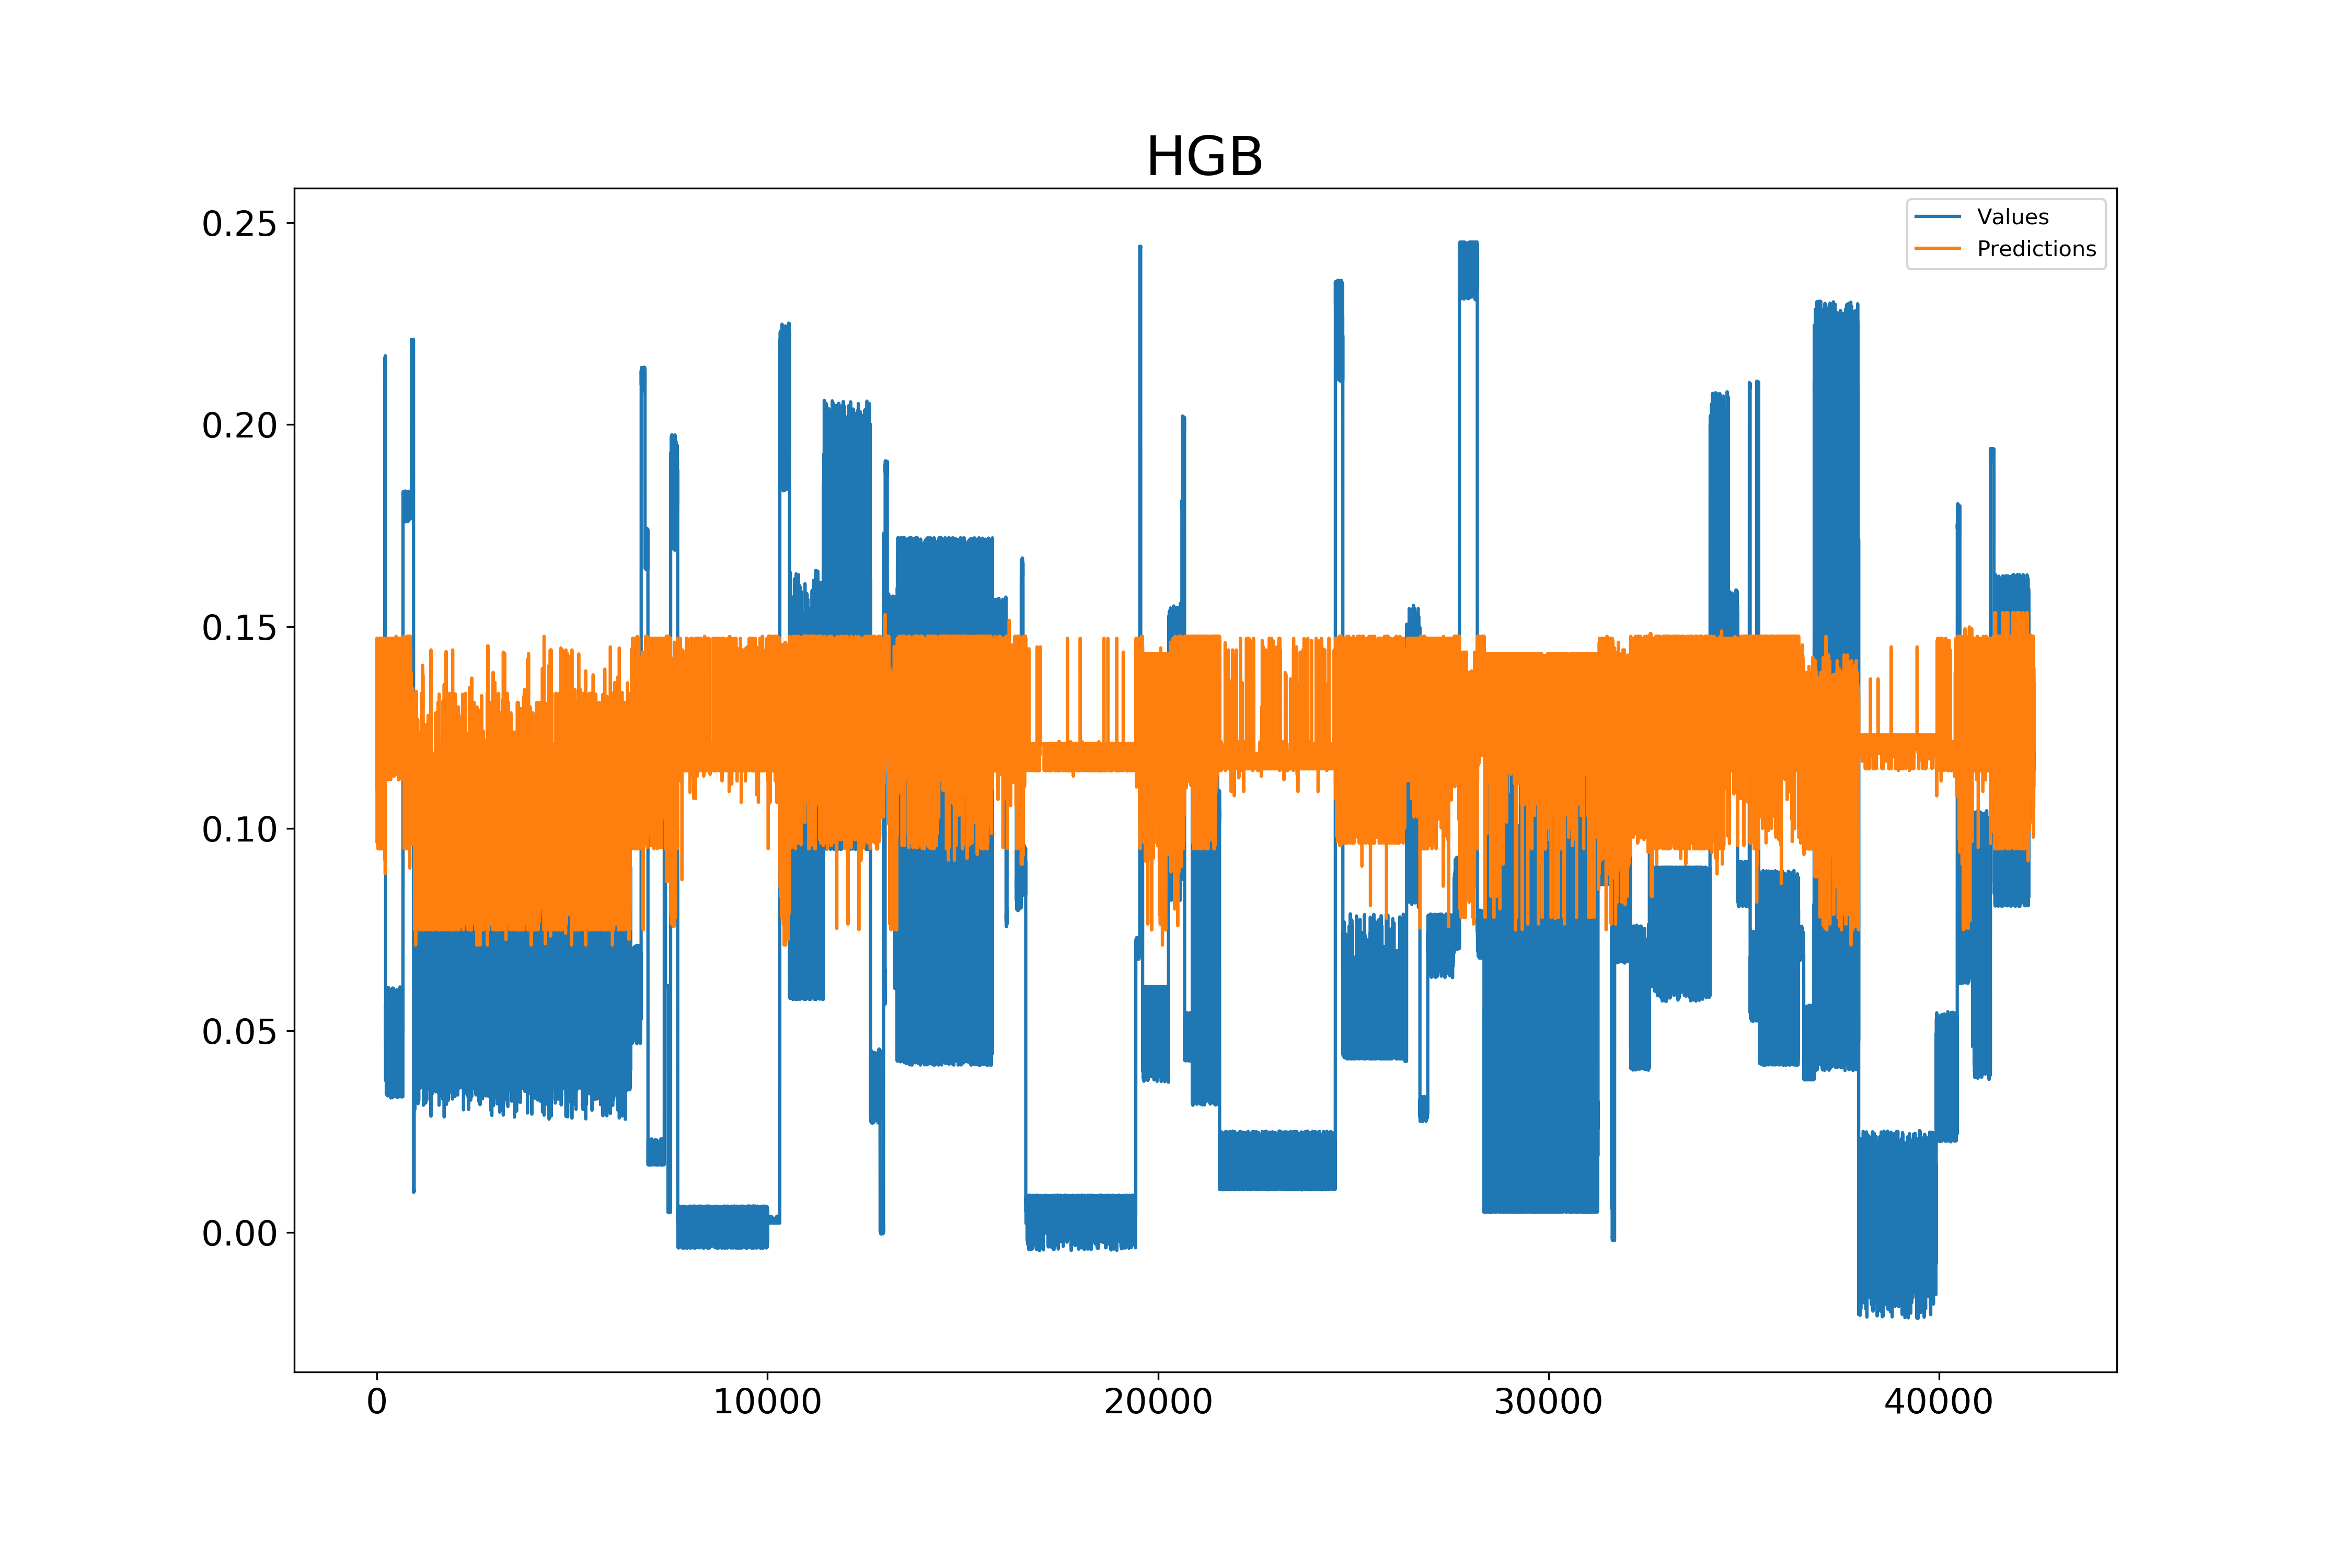
\includegraphics[width=\textwidth]{HGB_results}
		\caption{HistoryGradientBoosting}
	\end{subfigure}
	\begin{subfigure}{.24\textwidth}
		\centering
		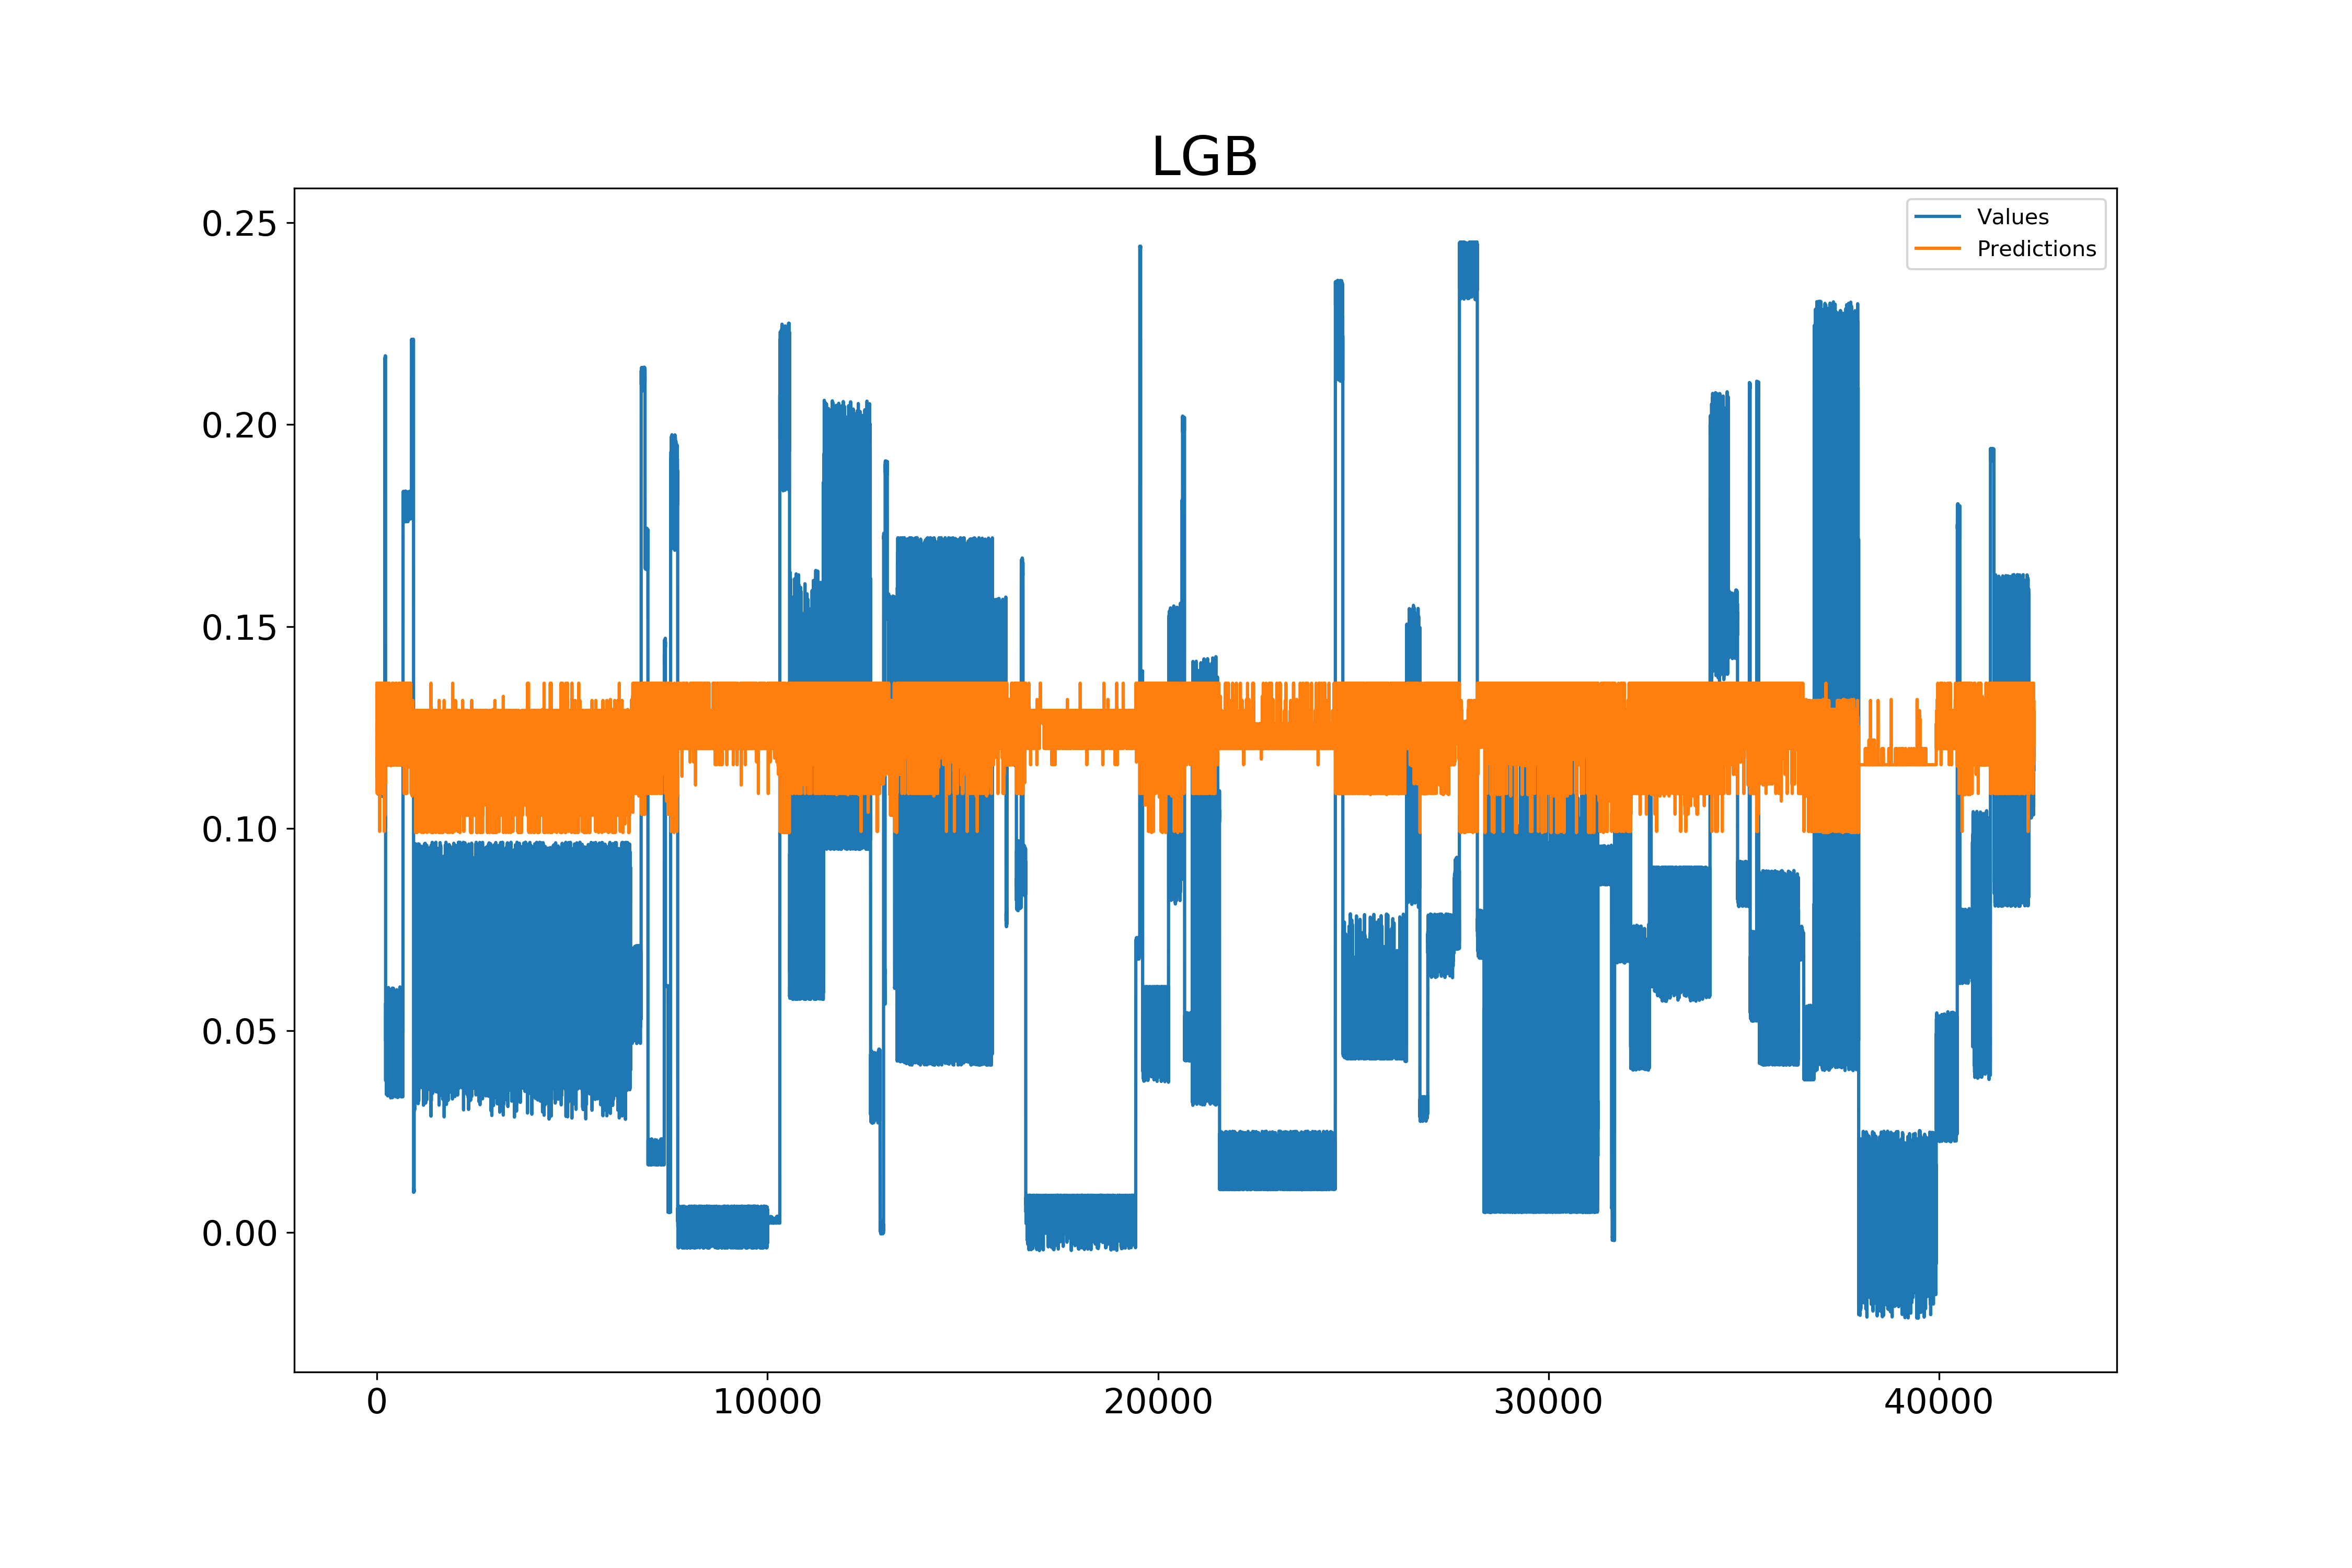
\includegraphics[width=\textwidth]{LGB_results}
		\caption{LightGBM}
	\end{subfigure}
	\begin{subfigure}{.24\textwidth}
		\centering
		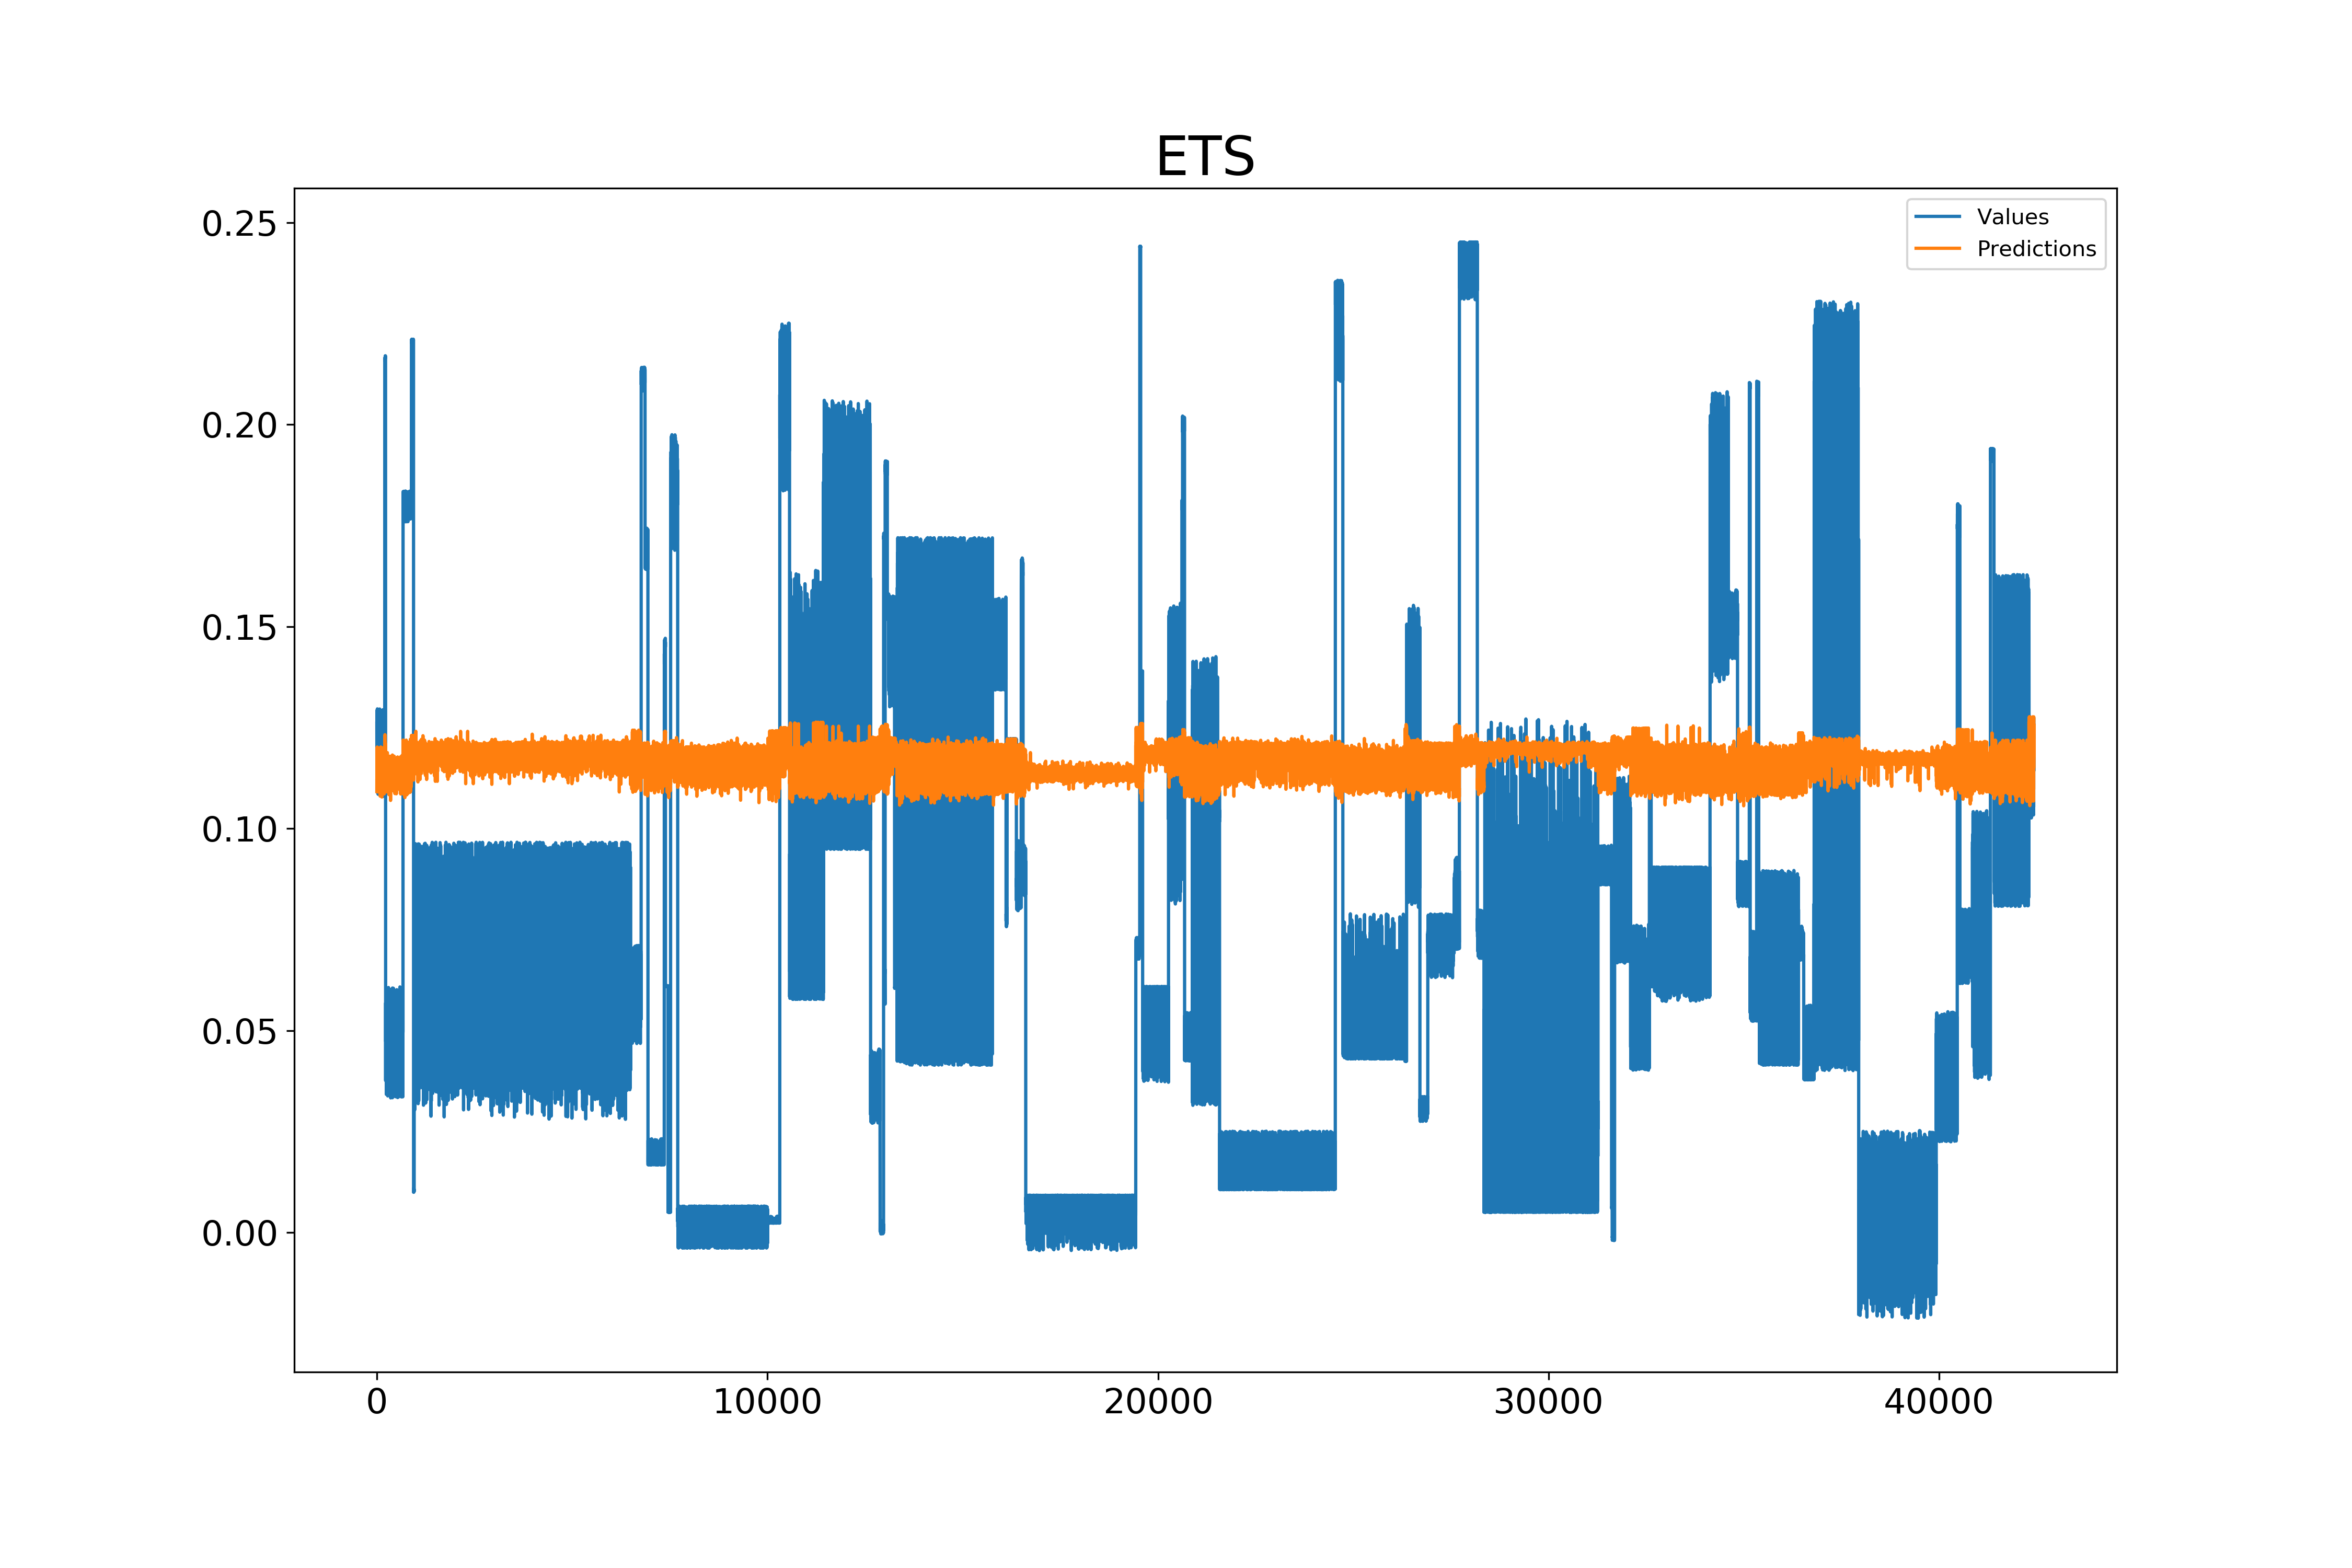
\includegraphics[width=\textwidth]{ETS_results}
		\caption{ExtraTrees}
	\end{subfigure}
	\caption{Comparison of concatenated predictions (orange) to ground truth (blue).}
	\label{fig:predictions}
\end{figure*}

Our results show that the regression is not able to differentiate between below and above the legal limit with the features extracted.

\subsection{Discussion}
We had a deadline to submit our results and in the mean time, the project continued to scale up as we progressed through different stages.
Thus, we had to compromise a bit of quality to gain speed and finish our project on time. These difficulties and compromises include the feature extraction where we could use more promising signal processing approaches to obtain better results.
More detailed description of this matter is further explained in the section \ref{sec:futurework}.

In the case of an application like this to become publicly accessible to users, there comes great responsibility with the data collection of the owners.
For one, this is extremely sensible data that could be trained to recognize even further information about an individual.
Another point is that in case the TAC level data gets leaked or sold to a third party, it could be abused to target the user with relevant ads or give drunk users higher transportation fares.
And finally, the app itself could produce defective detections, like a false negative resulting in irresponsible behavior while depending on a feedback from the application as an excuse to drive, for example.       

A direct comparison of the results of our trained regression model to the model proposed in \cite{DBLP:conf/ijcai/KillianPNMC19} is not possible, because not only did they not specify, on which chunks of the dataset they tested their trained models, they also performed a classification. And our regression has a more precise output and that results in worse metrics for our model, but does not necessarily represent the performance, because a threshold could be undershot by a tiny amount and would not necessarily mean a worse result, just a more precise one.

In addition to the aforementioned points, because this paper was created during a university course, many of our expectations couldn't be met because of strict time constraints.
If more time was available we could have increased our model performance by using details we discussed in the beginning of this section and chapter \ref{sec:futurework}.

\subsection{Conclusion}
Overall this project was a huge learning experience for all of us, and we learned a lot about data analysis. Additionally, we learned how fast a project can grow in dimension by adding more complexity and data. Furthermore we can conclude that in shallow machine learning algorithms the feature extraction has a huge impact on the model performance.

Our results were not meeting our expectations, but were of course limited by the time constraints of a university project and lacking the computational power to train more  models with the proposed changes. Otherwise, we see our whole pipeline of data analysis, cleaning and model tuning as a huge success.